\section{Fundamentals}
\label{sec:fundamentals}

\subsection{Raycasting}

Ray casting is primarily an imaging technique and was first described by Scott Roth in 1982 as an effective method of rendering CSG (Constructive Solid Geometry) objects. Although ray casting may be used for different purposes in various dimensions, we will focus on generating a two dimensional image from a three dimensional scene. The basic principle therefore is shown in figure \ref{fig:raycasting}. 

\begin{figure}
\centering
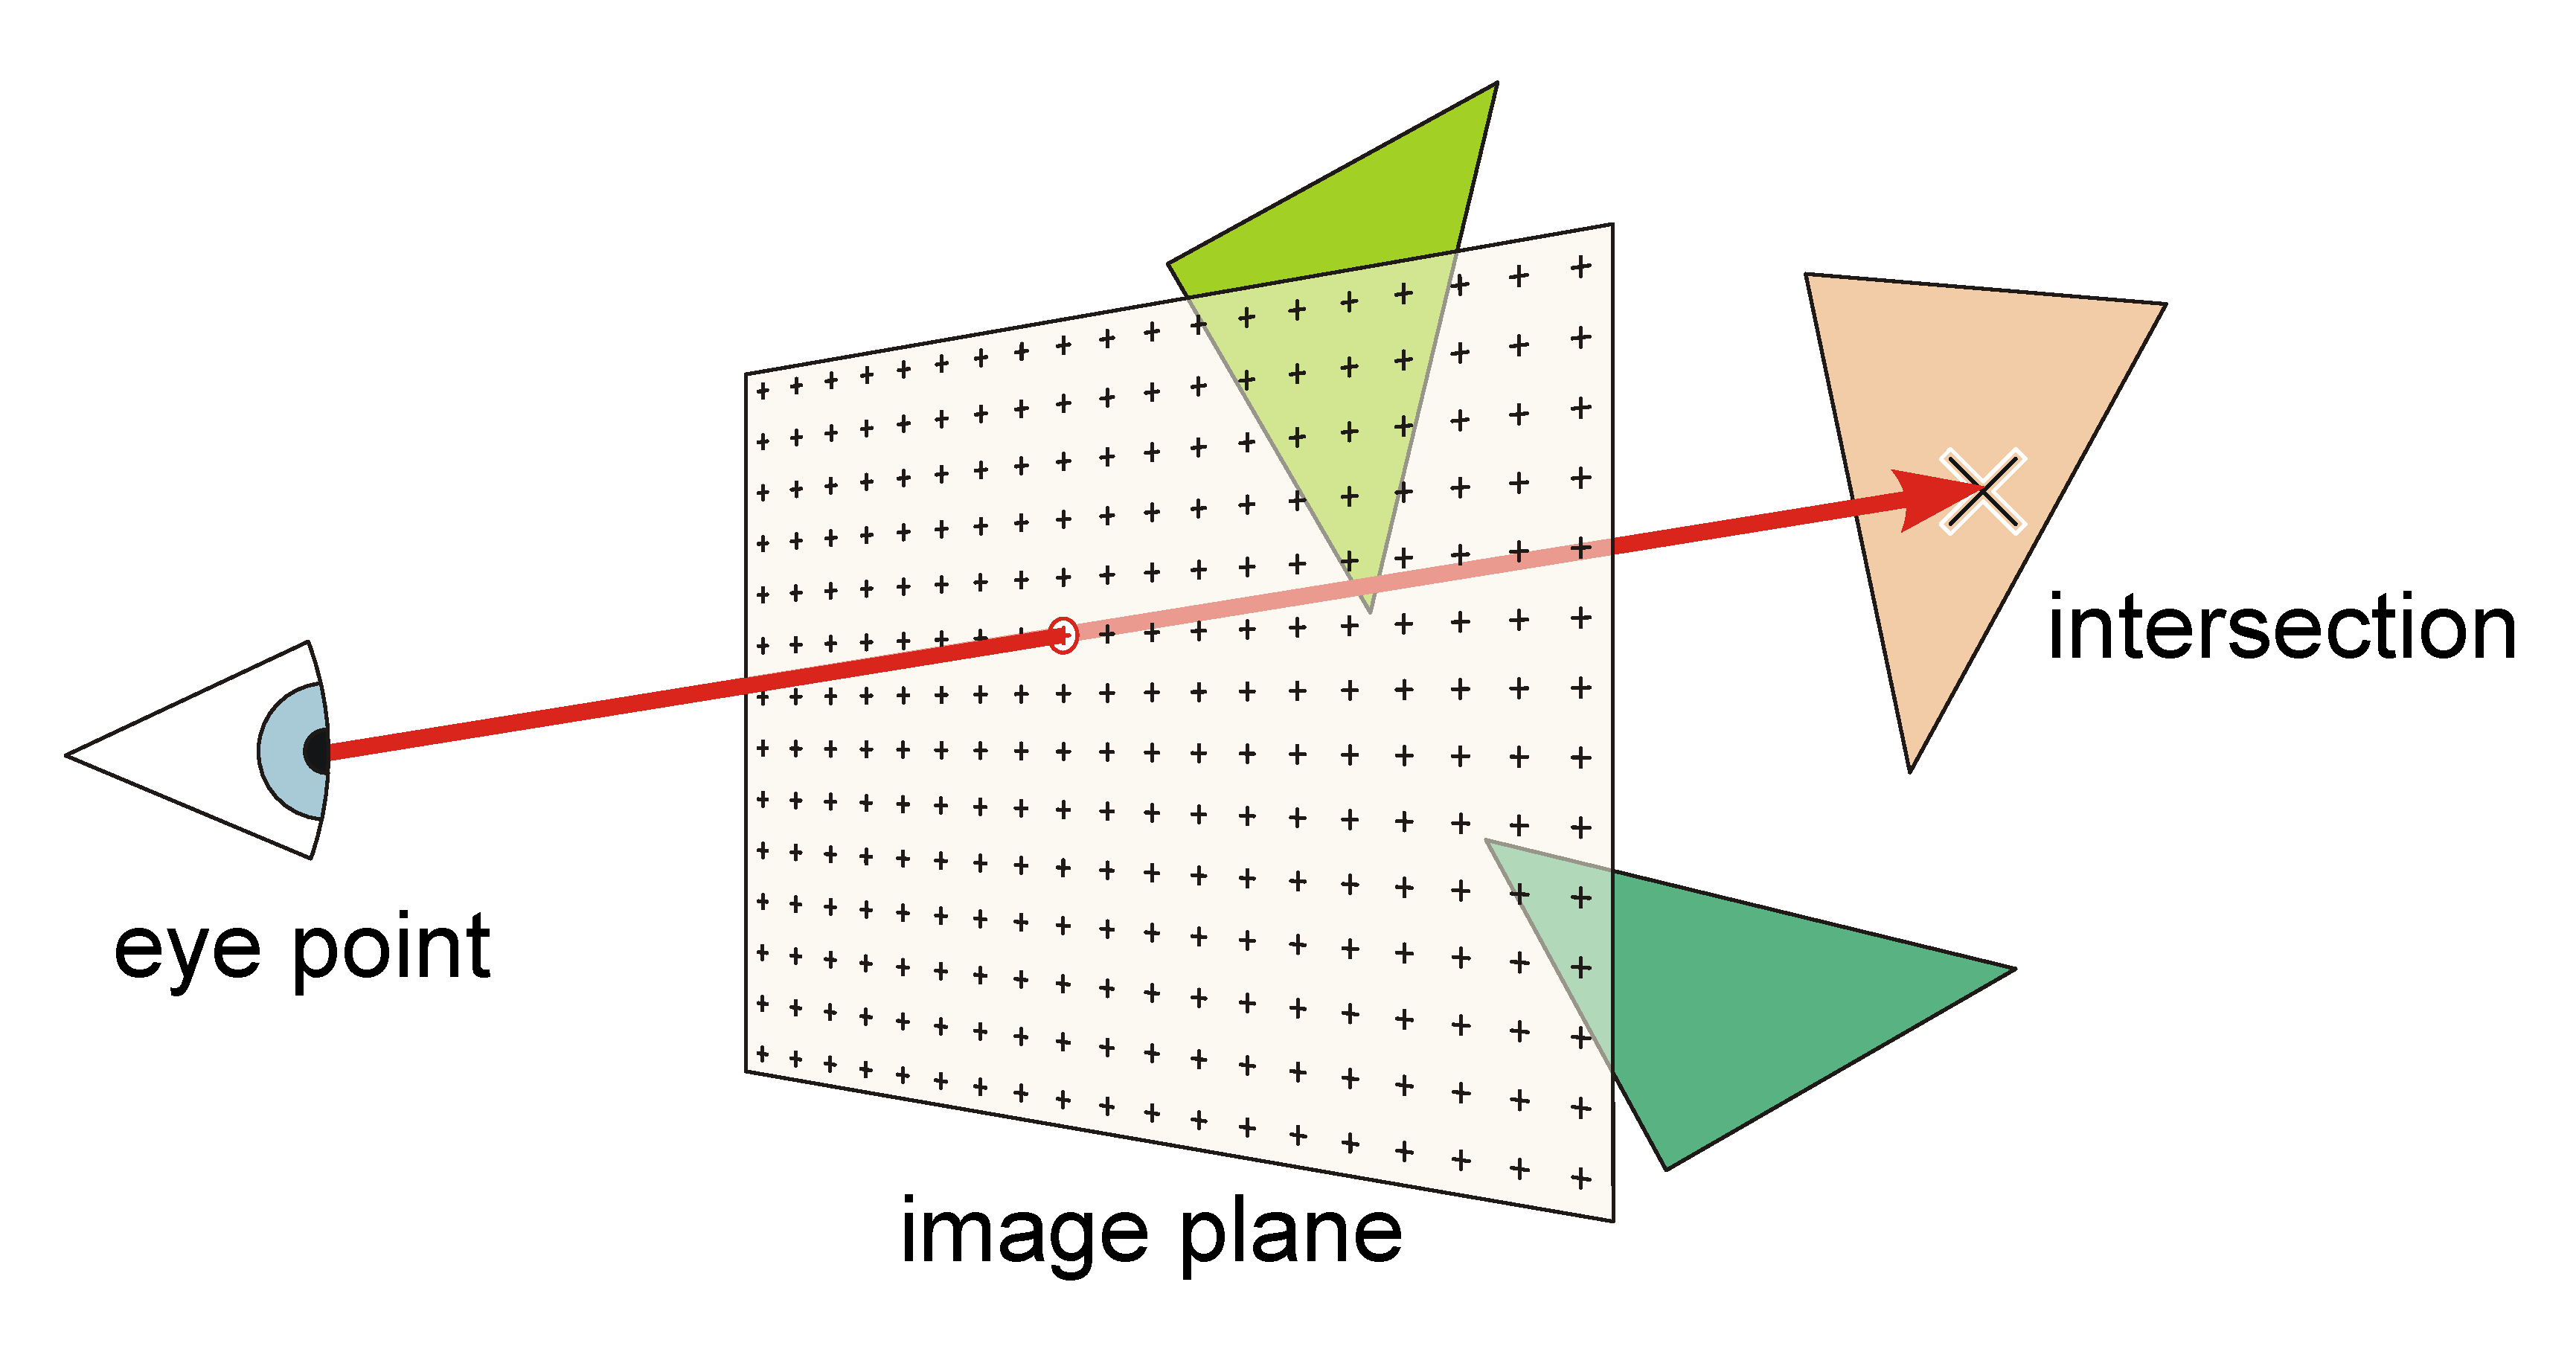
\includegraphics[width=0.6\linewidth]{raycasting}
\caption{Principle of ray casting.}
\label{fig:raycasting}
\end{figure}

Generating an image of a three dimensional scene of objects is done by sending rays from a defined eye point through the image plane into the scene. The image plain resembles the two dimensional output image which should be generated. Each output pixel is transformed into a three dimensional position on the image plane which is passed through by one ray originating from the eye point. The eye point itself is usually positioned centered before the image plane to achieve a perspective view of the scene. Each ray is then guided through the three dimensional space containing the scene objects trying to find an intersection. In the case an object is hit, a color value is calculated for the intersection point on the object (using e.g. materials parameters or textures of the surface). The pixel on the image plane, through which the ray was shot initially, is then set to this color.

Ray casting is different from the wide-spread rasterization used for most 3D applications and computer games today as it approaches from the image side instead of the objects, the scene is composed of. Rasterization takes all the objects placed in the scene (which have to be composed of primitive shapes, mostly triangles) and transforms them from three dimensional space to the two dimensional space of the output image where each object is then rasterized onto the pixels of the output image.

Apart a lot of technical differences, both methods also differ in complexity. Mark Kilgard describes the complexity of rasterization with $\mathcal{O}(b * m)$ whereas an accelerated ray tracing implementation (e.g. using a favorable data structure) achieves $\mathcal{O}(log b * p)$, where $b$ is the number of objects in the scene, $m$ is the average number of pixels per object and $p$ is the number of pixels in the scene \cite[p.48]{ray_casting_presentation}. The Enlight proposal additionally points out, that the size of computer screens increased far slower over the past decades than the size of computer memory, computational power and the size of industrial CAD (Computer-aided design) and CAM (Computer-aided manufacturing) models \cite{enlight_proposal}. Therefore, ray casting might be beneficial when used to render large scenes compost of huge amounts of triangles.


\subsection{Regular grids}

Regular grids are a type of data structure frequently used in ray casting/tracing to accelerate the traversal of rays through the scenes. Alternative approaches are often tree based such as kd trees, octrees, binary space partitioning (BSP) or bounding volume hierarchy (BVH). Each of these techniques has its own strengths and weaknesses depending on the scene and application. However, especially kd trees and grids (and multilevel grids) have been primarily focused in recent work about interactive ray casting/tracing \cite[ch.1]{packet_caster}. While kd trees usually perform amazingly well on static scenes, dynamic or animated objects still present a challenge as the used data structure has to be rebuilt after every scene change, which can take up to several seconds for larger sets of geometries \cite[ch.1]{packet_caster}. Regular grids are simpler structures for partitioning space and accelerating ray casting. They can be created quicker than a (balanced) tree, thus allowing more frequent scene changes. Nevertheless, kd trees may be up to a magnitude faster when it comes to the actual ray traversal \cite[ch.1]{packet_caster}. As Enlight focuses on visualizing dynamic scenes (for subtractive manufacturing) allowing at least ten subtraction volumes to be added to the scene per second, regular grids appear promising for being used in this case.

Building a regular grid data structure is simple. Initially, a bounding box is created around the scene. This box is then divided into equally sized cubes (which may force the box to be enlarged a bit to fit a whole number of cubes in each dimension) which are called cells. For each object (triangle) of the scene all spanned cells are calculated and the cells store a reference to the triangle.

During ray casting, the rays have to traverse the cells of the grid in order to find potential geometry they might intersect with. A fast algorithm for traversing regular grids using a single ray is given by John Amanatides and Andrew Woo \cite{3DDDA}. Their algorithm is a slight modification of the DDA (digital differential analyzer) which is used for the rasterization of lines. As finding the pixels (squares inside a regular 2D grid) which are covered by a line is actually the same problem as finding the voxels hit by a ray, this adapted 3D DDA algorithm can be used for efficient traversal of regular grids. Furthermore, as the algorithm's start point can be determined and the voxels (grid cells) are traversed incrementally, no depth sorting has to be performed across the hit cells and the traversal can be stopped on the first found intersection.



\subsection{Boolean raycasting}

works equal to CSG (Constructive Solid Geometry), except resulting mesh is never explicitly generated

water-tight

\subsubsection{Packet casting}

Casting 
different traversing

frustum culling
cache coherence (of adjacent rays)
SIMD




\subsection{OpenCL}

GPU hw architecture, how do kernels work? NDRange, buffers
